%%%%%%%%%%%%%%%%%%%%%%%%%%%%%%%%%%%%%%%%%%%%%%%%%%%%%%%%%%%%%%%%%%%%%%
% LaTeX Example: Project Report
%
% Source: http://www.howtotex.com
%
% Feel free to distribute this example, but please keep the referral
% to howtotex.com
% Date: March 2011 
% 
%%%%%%%%%%%%%%%%%%%%%%%%%%%%%%%%%%%%%%%%%%%%%%%%%%%%%%%%%%%%%%%%%%%%%%
% How to use writeLaTeX: 
%
% You edit the source code here on the left, and the preview on the
% right shows you the result within a few seconds.
%
% Bookmark this page and share the URL with your co-authors. They can
% edit at the same time!
%
% You can upload figures, bibliographies, custom classes and
% styles using the files menu.
%
% If you're new to LaTeX, the wikibook is a great place to start:
% http://en.wikibooks.org/wiki/LaTeX
%
%%%%%%%%%%%%%%%%%%%%%%%%%%%%%%%%%%%%%%%%%%%%%%%%%%%%%%%%%%%%%%%%%%%%%%
% Edit the title below to update the display in My Documents
%\title{Project Report}
%
%%% Preamble
\documentclass[paper=a4, fontsize=11pt]{scrartcl}

\usepackage[T1]{fontenc}
\usepackage{fourier}
\usepackage{times}
\usepackage{listings}
\usepackage{filecontents}

\usepackage[english]{babel}															% English language/hyphenation
\usepackage[protrusion=true,expansion=true]{microtype}	
\usepackage{amsmath,amsfonts,amsthm} % Math packages
\usepackage[pdftex]{graphicx}	
\usepackage{url}
\usepackage[bottom=0.5in]{geometry}

%%% Custom sectioning
\usepackage{sectsty}
\allsectionsfont{\centering \normalfont\scshape}


%%% Custom headers/footers (fancyhdr package)
\usepackage{fancyhdr}
\pagestyle{fancyplain}
\fancyhead{}											% No page header
\fancyfoot[L]{}											% Empty 
\fancyfoot[C]{}											% Empty
\fancyfoot[R]{\thepage}									% Pagenumbering
\renewcommand{\headrulewidth}{0pt}			% Remove header underlines
\renewcommand{\footrulewidth}{0pt}				% Remove footer underlines
\setlength{\headheight}{13.6pt}

%%% Equation and float numbering
\numberwithin{equation}{section}		% Equationnumbering: section.eq#
\numberwithin{figure}{section}			% Figurenumbering: section.fig#
\numberwithin{table}{section}				% Tablenumbering: section.tab#


%%% Maketitle metadata
\newcommand{\horrule}[1]{\rule{\linewidth}{#1}} 	% Horizontal rule

\title{
		%\vspace{-1in} 	
		\usefont{OT1}{bch}{b}{n}
		\normalfont \normalsize \textsc{Department of Computer Science, Technische Universit\"at Kaiserslautern\\
Compilers and Language Processing Tools - SS17
		} \\ [2pt]
		\horrule{0.5pt} \\[0.4cm]
		\huge A Parser and Lexer for Minijava\\
		\horrule{2pt} \\[0.5cm]
}

\author{	
		\textbf{Exercise 2}\\
		Group 03\\
        Daniele Gadler, Gopal Praveen\\Alka Scaria, Stephen Banin Payin \\[-1pt]		\normalsize
}


\date{May 13, 2017}

%%% Begin document
\begin{document}
\maketitle

\section*{Overview}
In the present report, we describe the parser we built for Minijava. More specifically, in the 'Features' section we explain what our parser is capable of doing, whereas in the 'Technical Description', we provide a deeper description of key components of the Parser.\\
 The constructed Parser passes all tests provided in the template as well as test cases laid out by the group members. It is also thoroughly documented by Javadoc. 
\subsection*{Features}

\begin{itemize}
	\item \textbf{Abstract Syntax Tree Construction}: The parser is capable of parsing java files according to the grammar given as part the exercise and representing a Java file's structure as an AST. \\
Figure \ref{classPic} shows how the parser is able to parse nested structures and represent them as an AST.

\begin{figure}[h]
	 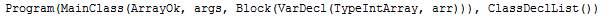
\includegraphics[scale=1]{class.png}
	 \caption{Resulting AST for a java class containing an array declaration in the main method.}
	 \label{classPic}
\end{figure}

	\item \textbf{Invalid statements recognition}:  The parser disallows the parsing of expressions that are not allowed in Java within a statement. This is carried out for stray expressions (Statement --> Exp;) and assignment expressions (Statement --> Exp = Expr;).\\
	 Upon encountering invalid statements, the parser catches the latter and raises appropriate syntax errors.\\ For example, when parsing the following expression contained in a valid method "2 = id", the following syntax error will be raised:
	 
	\textit{The left-hand side of an assignment expression cannot be a number.}

\end{itemize}

\section*{Technical Description}

\subsection*{Task 1: Grammar implementation, Operator precedence and associativity }
\label{Task1}

We implemented the grammar for parsing Minijava as described in the exercise's grammar specifications: particular attention needed to be paid to the implementation of following elements: 
\begin{itemize}
	\item \textbf{Kleene Star (*)}: The Minijava elements  that may appear zero or more times (e.g: ClassDecl, MemberDecl, BlockStatement, ExprRest) as lists. \\
	Lists' wrapping of elements was implemented in a recursive manner: firstly, it was checked if an element of the list is followed by a list of elements and parse the single element found.  After the element is parsed, it is added to the list of elements parsed so far and the other elements in the list are parsed in the same recursive manner. If a list appears to empty, an empty list is returned. 
%A particular case is represented by the implementation of a list of statements (MJStatement), which does not posses any default list's implementation: in this case, we returned an empty LinkedList if the list was detected to be empty.  
	\item \textbf{Optional (?)}: The optional Minijava elements that may appear zero or one time (e.g: ExprList, ParaList) as lists. \\
	If such a list appears to contain valid element(s), then it is parsed. Alternatively, if such a list is recognized to be empty, then an empty list is returned. The main difference between 'optional' lists and 'Kleene star' lists lies in the fact that optional lists are parsed just one time, no matter they are empty or contain something. 
\end{itemize}

The operators' precedence and associativity were implemented by grouping expressions' operations' declarations into the same grammar declaration. By doing so, operators' precedence declarations can actually have an effect on the associativity and the order of operations. Consequently, we declared the following precedence rules for Java operators, as described by \cite{Princeton}.


\begin{lstlisting}
precedence left EQ;
precedence left AND;
precedence left EQUALS;
precedence left LESS;
precedence left PLUS, MINUS;
precedence left TIMES, DIV;
precedence left LBRACKET, RBRACKET, DOT, LPAREN, RPAREN;
\end{lstlisting}


\subsection*{Task 2 - Invalid Statements Recognition}

We implemented invalid statements' recognition by making use of the visitor pattern in the MJInvalidStatement class. By passing the AST constructed in Task 1 to  the "acceptProgram" method, the whole tree is traversed with the purpose of detecting statements that are invalid in Java.\\
By overriding the visit method for \textbf{assignment statements} (e.g.: Statement --> Expr = Expr;), we raise appropriate syntax errors if the left-hand side of assignment operations contains: a number, a binary expression, 'this', 'null', an array length expression, a unary expression (!Expr or -Expr) or a boolean constant.\\
We also overrode the visit method for \textbf{'stray' expressions} (e.g.: Statement --> Expr;). The only stray expressions allowed are 'MethodCall' and 'New Object Creation'. In all other cases, a syntax error is raised. 

\begin{thebibliography}{9}% 2nd arg is the width of the widest label.
\bibitem{Princeton}
Precedence and associativity of Java operators. \textit{http://introcs.cs.princeton.edu/java/11precedence/}. Accessed on 10th May 2017.
\end{thebibliography}

\end{document}